
\section{Bobby Mira}

\begin{rpg-pcbox}{Bobby Mira}{img/bobby-mira.png}
    The veteran firefighter in the crew. You grandfather was a firefighter, your father was a firefighter. You are a firefighter. It runs in the blood, but that doesn't mean that you are in the job for the joy of saving lives. Half the people in the station are just straight up idiots who are alive by the sole miracle of industrial/insurance companies doing the bare minimum so that the stupid people don't die and they have to pay for their stupidity. Well you get the idea.
\end{rpg-pcbox}

\begin{rpg-commentbox}{}
    Roughneck

    \textbf{STRENGTH} 5, \textbf{AGILITY} 4, \textbf{WITS} 3, \textbf{EMPATHY} 2

    \textbf{HEALTH}: 5

    \textbf{SKILLS}: Heavy Machinery 2; Close combat 1; Stamina 2; Mobility 2; Observation 2; Comm tech 1;
    
    \textbf{TALENT}: True grit
    
    \textbf{GEAR}: Cutting Torch;
    
    Maintenance jack (haligan);
    
    M314 Motion tracker;
    
    MK.60 suit---Armor Rating 2. Max Air supply 6;  
    
    Tool belt (signature)

    
    \textbf{BUDY}: Anderson
    
    \textbf{RIVAL}: Lice or Ronda
\end{rpg-commentbox}


\begin{rpg-commentbox}{Agenda}
    \begin{enumerate}[label=\textbf{Act \arabic*}, leftmargin=1cm]
        \item Don't deviate from the plan. Ensure that your crew stick to the chief's orders 
        \item No heroic shit. Clean sedation ward and get out. Don't confront the alien
        \item Weyland-Yutani has our best interest. Cooperate with the mercenaries
    \end{enumerate}
\end{rpg-commentbox}


% \makebox[0pt][l]{%
%   \raisebox{-\totalheight}[0pt][0pt]{%
%     \vspace*{200in}%
%     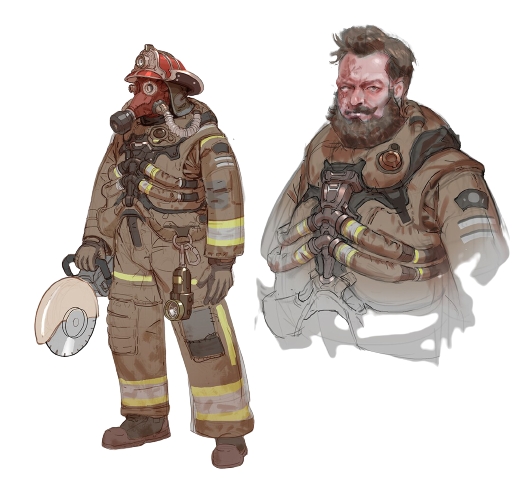
\includegraphics[width=.70\textwidth]{img/bg/firefighter-1.png}}}%

% \begin{figure}
%     \centering
%     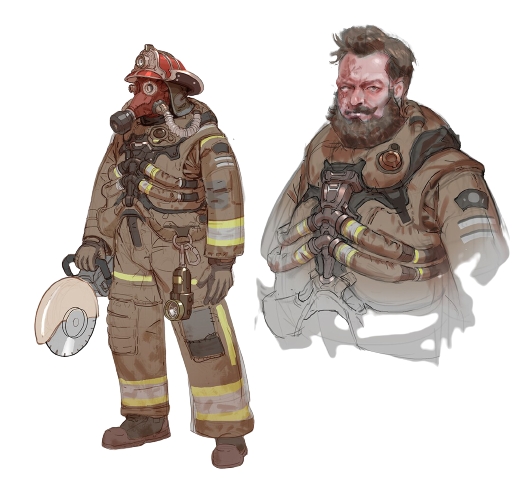
\includegraphics[width=.50\textwidth]{img/bg/firefighter-1.png}
%     \label{fig:refinery}
% \end{figure}


\begin{figure}
    \centering
    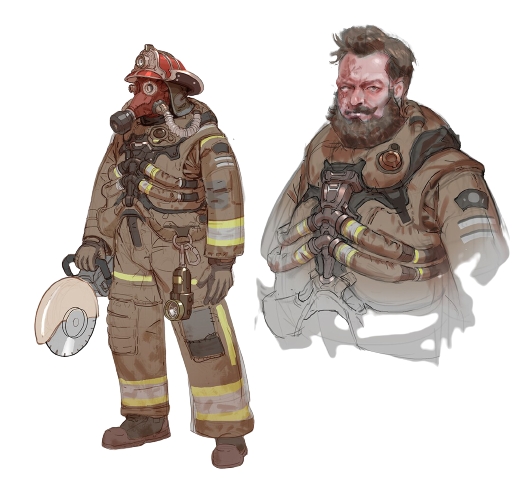
\includegraphics[width=.45\textwidth]{img/bg/firefighter-1.png}
    \label{fig:refinery}
\end{figure}

\newsect

\clearpage


\section{Connor Scofield}

\begin{rpg-pcbox}{Connor Scofield --- \texttt{\textbf{u/\_ArthurDallas\_}}}{img/connor-scofield.png}
    An ex colonial marine with nerves of steel. He has done it all and saw everything twice. His past commander was brutally murdered in a sabotage routine military mission. Connor suspected an enemy under cover, but as soon as he started asking too many questions, they pushed him out to resign. Connor suspects a Weyland-Yutani agent for the crime and he's gonna find them...
    
\end{rpg-pcbox}

\begin{rpg-commentbox}{}
    Ex-Marine

    \textbf{STRENGTH} 4, \textbf{AGILITY} 4, \textbf{WITS} 3, \textbf{EMPATHY} 4

    \textbf{HEALTH}: 4

    \textbf{SKILLS}: Heavy Machinery 2; Close combat 1; Stamina 1; Mobility 1; Observation 2; Comm tech 2; Command 1; Manipulation 1; Ranged combat 1;
    
    \textbf{TALENT}: Nerves of Steel
    
    \textbf{GEAR}: Cutting Torch;
    
    Maintenance jack (haligan);
    
    Hydraulic Rescue tool (spreader);
    
    MK.60 suit---Armor Rating 2. Max Air supply 6;  
    
    dog tags (signature)
      
    \textbf{BUDY}: Bobby
    
    \textbf{RIVAL}: Lice
\end{rpg-commentbox}


\begin{rpg-commentbox}{Agenda}
    \begin{enumerate}[label=\textbf{Act \arabic*}, leftmargin=1cm]
        \item Find anything that can link Weyland-Yutani to the fire in the facility
        \item Recover one of the data drivers that has info about the mysterious room
        \item Uncover whether the mercenaries are friend or foe
    \end{enumerate}
\end{rpg-commentbox}


\newsect

\begin{figure}
    \centering
    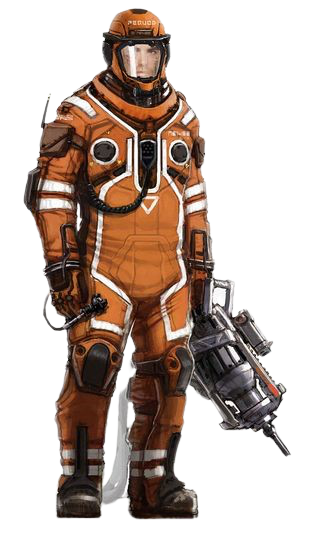
\includegraphics[width=.45\textwidth]{img/bg/firefighter-2.png}
    \label{fig:refinery}
\end{figure}


\clearpage

\section{Dave Colt}

\begin{rpg-pcbox}{Dave Colt}{img/dave-colt.png}
    The paramedic of the crew. You are usually the one that bring the bad news that someone's limbs will need amputation but regardless, it's the only place where you can practice medicine. Besides, you get real pleasure in doing all the amputation/gore work. It's not like you won't accidentally kill one or two people with an overdose.
    Anywhere else, you would be flagged as a creep. Here, you transpire competence and whoever died in one of your shifts is just another junkie who is better of dead. Your competence speaks louder than these casualties.
\end{rpg-pcbox}

\begin{rpg-commentbox}{}
    Scientist

    \textbf{STRENGTH} 3, \textbf{AGILITY} 3, \textbf{WITS} 4, \textbf{EMPATHY} 4

    \textbf{HEALTH}: 3

    \textbf{SKILLS}: Heavy Machinery 1; Close combat 1; Stamina 2; Mobility 3; Observation 2; Comm tech 1; Medical Aid 3;
    
    \textbf{TALENT}: Field Surgeon
    
    \textbf{GEAR}: Maintenance jack (haligan);
    
    MedKit;

    D6 does of NAPROLEVE;
    
    MK.60 suit---Armor Rating 2. Max Air supply 6;  
    
    Trinket from his last victim (signature)

    \textbf{BUDY}: Anderson
    
    \textbf{RIVAL}: Connor
\end{rpg-commentbox}


\begin{rpg-commentbox}{Agenda}
    \begin{enumerate}[label=\textbf{Act \arabic*}, leftmargin=1cm]
        \item We need some air. Gather emergency supplies in anticipation for the worst!
        \item We need to keep it cool. Convince others that you need more NAPROLEVE and that going back to the pharmacy is worth the risk.
        \item We can kill it! Jeopardize the efforts of your crew on trying to kill the alien. One example is to add NAPROLEVE in the extra air supply of your crew members so that they overdose while you escape.
    \end{enumerate}
\end{rpg-commentbox}

\newsect


\section{Anderson Rice}

\begin{rpg-pcbox}{Rice Anderson}{img/Rice-Anderson.png}
    You are still under probation. Trying to secure a job and provide for your family is your priority. A dedicated mormon, you want to use firefighting to connect to victims of accidents and put them in the path to salvation. Little you know that your faith will soon be put to test. \texttt{\textbf{IMPORTANT}} this is NOT a comical joke on a certain religion group but rather the idea of exploring faith in a horror setting. 
\end{rpg-pcbox}

\begin{rpg-commentbox}{}
    Roughneck

    \textbf{STRENGTH} 4, \textbf{AGILITY} 5, \textbf{WITS} 2, \textbf{EMPATHY} 3

    \textbf{HEALTH}: 4

    \textbf{SKILLS}: Heavy Machinery 1; Close combat 1; Stamina 2; Mobility 2; Observation 2; Comm tech 1; Command 1; Manipulation 1;
    
    \textbf{TALENT}: Calm Breather
    
    \textbf{GEAR}: Cutting Torch;
    
    Maintenance jack (haligan);
    
    Rescue breather---Air supply 2;
    
    MK.60 suit---Armor Rating 2. Max Air supply 6;  
    
    Letter from a of Mormon pastor (signature)

    \textbf{BUDY}: Ronda
    
    \textbf{RIVAL}: Bobby
\end{rpg-commentbox}


\begin{rpg-commentbox}{Agenda}
    \begin{enumerate}[label=\textbf{Act \arabic*}, leftmargin=1cm]
        \item While in the firetruck or fire station, convince another crew member to go to a bible study with you later
        \item I have sinned! Tell to one of your crew mates an horrible sin that you have committed --- this might have implications on stealth mode
        \item For my family. Save the rest of the crew even if that means your death. 
    \end{enumerate}
\end{rpg-commentbox}


\newsect

\clearpage

\section{Jordan Zemke}


\begin{rpg-pcbox}{Jordan Zemke}{img/jordan-zemke.png}
    You dreamed of becoming a pilot and flying a Cheyenne dropship. Reality punched you hard and you are stick in this hell of a job. You promised you would get into something better, you made this same promise  for the past 8 years... at least you can drive the firetruck.
\end{rpg-pcbox}

\begin{rpg-commentbox}{}
    Pilot

    \textbf{STRENGTH} 3, \textbf{AGILITY} 5, \textbf{WITS} 4, \textbf{EMPATHY} 2

    \textbf{HEALTH}: 4

    \textbf{SKILLS}: Heavy Machinery 2; Close combat 1; Stamina 2; Mobility 2; Observation 2; Comm tech 2; Piloting 2;

    \textbf{TALENT}: Fast Reflexes
    
    \textbf{GEAR}: Cutting Torch;
    
    Maintenance jack (haligan);
    
    Seegson system diagnostic device;
    
    MK.60 suit---Armor Rating 2. Max Air supply 6;  
    
    Pilot shades (signature)

    \textbf{BUDY}: Dave
    
    \textbf{RIVAL}: Connor
\end{rpg-commentbox}


\begin{rpg-commentbox}{Agenda}
    \begin{enumerate}[label=\textbf{Act \arabic*}, leftmargin=1cm]
        \item Get drugs in the facility pharmacy
        \item If someone is gonna die, that ain't me. If any of your comrades decides to confront the alien, you will do your best to stay away from action or even push some of your friends towards the creature so you can stay safe.
        \item I won't die like this. Fake your death so that you can escape after things cool down.
    \end{enumerate}
\end{rpg-commentbox}


\begin{figure}
    \hspace*{-1in}
    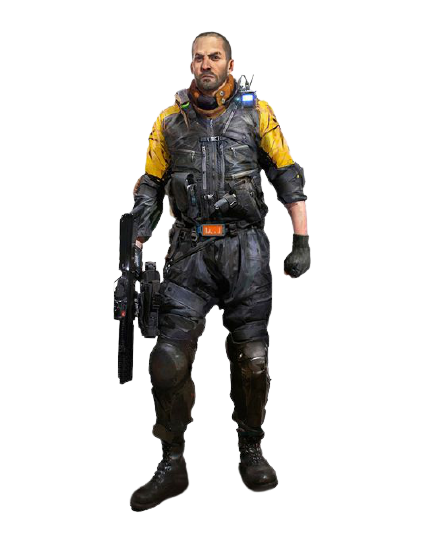
\includegraphics[width=.65\textwidth]{img/bg/firefighter-6.png}
    \label{fig:refinery}
\end{figure}


\newsect

\clearpage



% \makebox[0pt][l]{%
%   \raisebox{-\totalheight}[0pt][0pt]{%
%     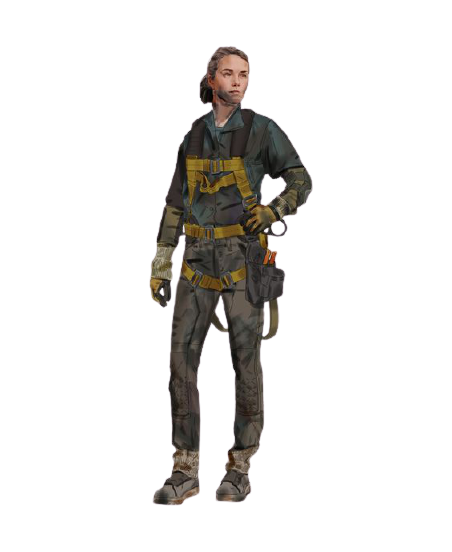
\includegraphics[width=.85\textwidth]{img/bg/firefighter-5.png}}}%


\section{Lice Coly}

\begin{rpg-pcbox}{Lice Coly --- \texttt{\textbf{u/\_ArthurDallas\_}}}{img/lice-coly.png}
    She's recklesss, living for the rush of adrenaline. Lice can put a really strong facade to someone that is in fact desperate/bankrupt. All the reckless is just to hide all her concerns about her little brother's multiple organ failures. He is dying and she must find something to get her enough money to save her only family.
\end{rpg-pcbox}

\begin{rpg-commentbox}{}
    Roughneck

    \textbf{STRENGTH} 3, \textbf{AGILITY} 3, \textbf{WITS} 4, \textbf{EMPATHY} 4

    \textbf{HEALTH}: 3

    \textbf{SKILLS}: Heavy Machinery 2; Ranged combat 1; Stamina 2; Mobility 1; Observation 2; Comm tech 2; Manipulation 2;
    
    \textbf{TALENT}: Reckless
    
    \textbf{GEAR}: Cutting Torch;
    
    Maintenance jack (haligan);
    
    Rescue Breather---Air supply 2;
    
    MK.60 suit---Armor Rating 2. Max Air supply 6;  
    
    LEGO toy from her brother (signature)

    \textbf{BUDY}: Jordan
    
    \textbf{RIVAL}: Connor
\end{rpg-commentbox}

\begin{rpg-commentbox}{Agenda}
    \begin{enumerate}[label=\textbf{Act \arabic*}, leftmargin=1cm]
        \item Ensure that the ICU where her brother is is not vent and that her brother is safe
        \item Recover one of the data drivers that has info about the mysterious room
        \item Negotiate her safety with the mercenaries so that she can save herself and her brother. Screw the rest of the crew!
    \end{enumerate}
\end{rpg-commentbox}


\begin{figure}
    \hspace*{-1in}
    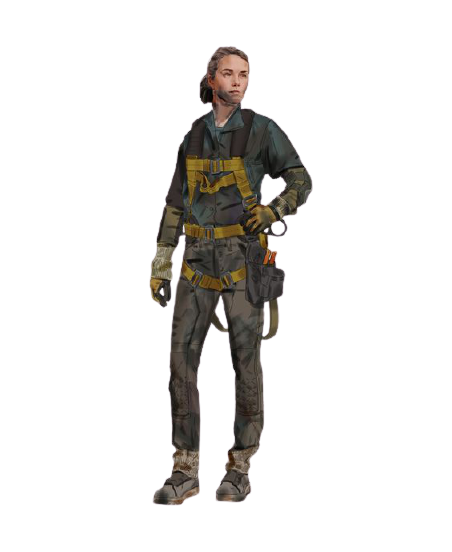
\includegraphics[width=.7\textwidth]{img/bg/firefighter-5.png}
    \label{fig:refinery}
\end{figure}


\newsect

\clearpage

\section{Ronda Gonzalez}

\begin{rpg-pcbox}{Ronda Gonzalez}{img/ronda-gonzalez.png}
    The badass mechanic of the crew. If it has screws, you can disassemble and assemble it back in no time. You have the respect of half the roughnecks in the station and you have saved their lives more than once. 
\end{rpg-pcbox}

\begin{rpg-commentbox}{}
    Roughneck

    \textbf{STRENGTH} 5, \textbf{AGILITY} 4, \textbf{WITS} 3, \textbf{EMPATHY} 2

    \textbf{HEALTH}: 5

    \textbf{SKILLS}: Heavy Machinery 2; Close combat 1; Stamina 2; Mobility 2; Observation 2; Comm tech 3;
    
    \textbf{TALENT}: Cunning
    
    \textbf{GEAR}: Maintenance Jack (haligan);
    
    Seegson diagnostic device;
    
    Hydraulic rescue tool (spreader);
    
    MK.60 suit---Armor Rating 2. Max Air supply 6;  
    
    Family photo (signature)

    \textbf{BUDY}: Connor
    
    \textbf{RIVAL}: Bobby
\end{rpg-commentbox}


\begin{rpg-commentbox}{Agenda}
    \begin{enumerate}[label=\textbf{Act \arabic*}, leftmargin=1cm]
        \item Make sure that no corridor is vented with a roughneck on it.
        \item For the greater good! Convince others to kill the alien in the mortage furnace
        \item This thing will not leave this place. Do all that you can to not let the alien escape the facility. Ask MU/TH/UR about ``who blinks first?''
    \end{enumerate}
\end{rpg-commentbox}


\newsect

\begin{figure}
    \centering
    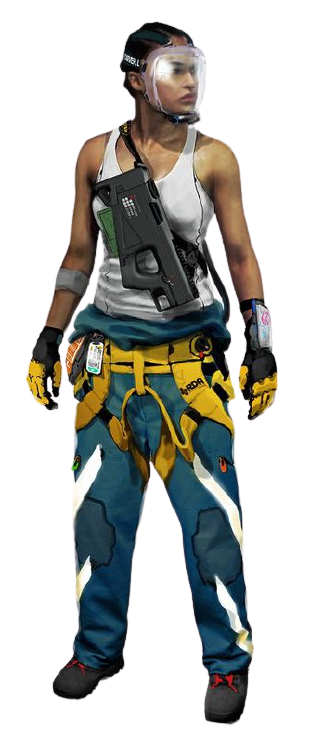
\includegraphics[width=.35\textwidth]{img/bg/firefighter-4.png}
    \label{fig:refinery}
\end{figure}




\clearpage

